\newpage
\section{Ordinary Least Squares}
This section will introduce the method of ordinary least squares for estimating parameters in a linear regression model.

\subsection{Least Squares}
The main idea behind the least squares is to minimize the sum of squared residuals, also known as SSR. 
Given a set of data points in the plane how might one find the line that best fit the data, one way is to choose the line that minimizes the sum of squared residuals.
In figure \ref{fig:example_simple_linear_regression} an example of a simple linear regression can be seen. 
The figure illustrates the log price plotted against the age of property sold by Home in Aalborg within the year 2012.
\begin{figure}[h]
    \centering
    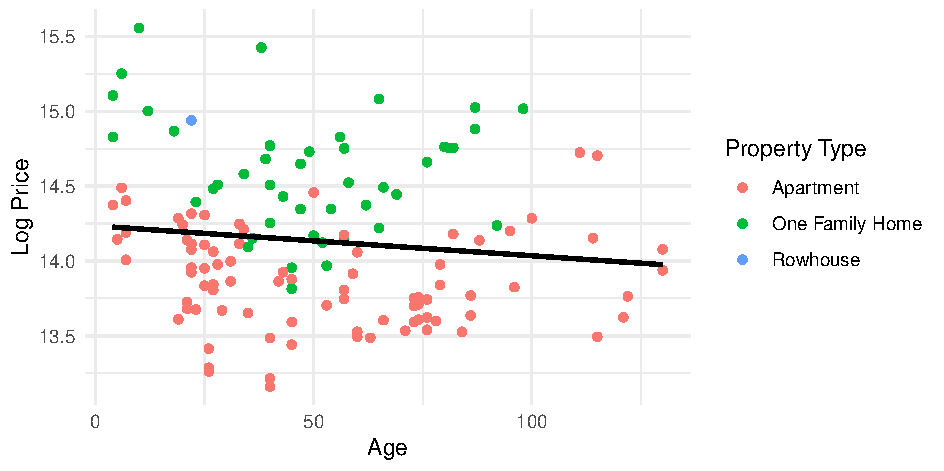
\includegraphics[width = 0.9\textwidth]{figures/Ordinary_Least_Squares/example_linear_regression.pdf}
    \caption{Age and log price of property sold in 2012 by Home in Aalborg.}
    \label{fig:example_simple_linear_regression}
\end{figure}

The dataset has observations of the form $\{a_i, log(p_i)\}$ with $i = 1, \ldots, 130$. The age of property is seen as the independent variable and the log price as the dependent variable.
We can assume, albeit naive considering figure \ref{fig:example_simple_linear_regression}, that there is a linear relationship between age and log price of the property in question.
This can be formulated as
\begin{align}\label{eq:approx_linear_relationship}
    log(p) \approx \beta_0 + \beta_1 a
\end{align}
where $log(p)$ and $a$ denotes the log price and age respectively.
The right side \eqref{eq:approx_linear_relationship} is the model function in our case.
The function is on the form $f(a, \boldsymbol{\beta})$, where $\boldsymbol{\beta}$ is a $2 \times 1$ vector containing the parameters $\beta_0$ and $\beta_1$.
The goal is now to find $\boldsymbol{\beta}$ that minimizes the sum of squared residuals.
For the $i$'th observation the residual is defined as $r_i = log(p_i) - f(a, \boldsymbol{\beta})$.
With the notation in place we can now write the sum of squared residuals as
\begin{align}\label{eq:SSR}
  SSR = \sum_{i = 1}^{130} r_i^2 = \sum_{i = 1}^{130} \left( log(p_i) - f(a, \boldsymbol{\beta}) \right)^2
\end{align}


